\section{Background}

\begin{frame}{Information Flow and Access Control}
	Many systems control access to information with \textbf{access control} mechanisms, which place restrictions based on the \textit{permissions} of a user or of calling code, but which cannot restrict how that information \textit{propagates} once released \cite{ifbackground:sabelfeld}.
	
	\textbf{Information flow} mechanisms instead control access by enforcing that some \textit{policy} on the data is upheld.
	
	In short, access control puts controls on the \textit{calling code}, where information flow puts controls on the \textit{data}.
\end{frame}

\begin{frame}{Information Flow Basics}
	In its most general form, information flow security considers confidentiality states. An information flow policy formalises how information may move between states.
	
	This is commonly represented by applying the Bell-LaPadula Lattice model used in Mandatory Access Control.
	
	\begin{figure}
		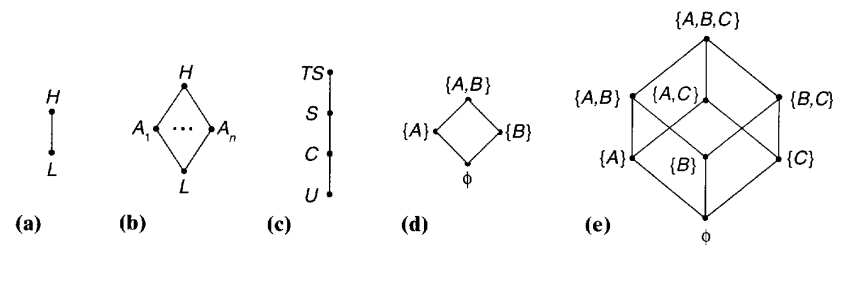
\includegraphics[scale=0.45]{content/images/lattice_examples.png}
		\caption{Example Lattice Model policies \cite{ifbackground:sandhu}}
	\end{figure}
	
\end{frame}

\begin{frame}{Noninterference}
	\begin{block}{Noninterference}
		``A group of users [or a program] is noninterfering with another group of users if what the first group does with those commands has no effect on what the second group of users can see."\newline \tiny{-- Goguen \& Meseguer} \cite{ifbackground:goguen}
	\end{block}
	
	Information flow models attempt to verify that programs have the property of \textit{noninterference} -- that is, if two executions of the program are identical in their low confidentiality inputs, then their behaviour should be indistinguishable from each other to an attacker.
	
	A noninterfering program \textit{provably} protects confidentiality.
\end{frame}

\begin{frame}{Noninterference - Is It Practical?}
	If we can verify the flows of information through a program, we can prove that it is noninterfering, but there are two serious problems with attempting to do so:
	
	\begin{enumerate}
		\item Proving non-interference is undecidable
			\begin{itemize}
				\item The halting problem can be reduced to it -- consider: \newline \texttt{\textbf{if} S() halts \textbf{then} h := 1 \textbf{else} h := 0} \cite{ifbackground:denninghalting}
				\item We \textit{can} build tools which reject all interfering programs, with the cost that some noninterfering programs are also rejected 
			\end{itemize}
		\item Many useful programs are inherently interfering
			\begin{itemize}
				\item A password checker's output clearly depends on the password
			\end{itemize}
	\end{enumerate}
\end{frame}

\begin{frame}{Practical Noninterference}
	The second problem means almost any real world program cannot be noninterfering. So most practical information flow solutions do not require true noninterference. Instead, they may:
	
	\begin{itemize}
		\item Allow `selective declassification' of confidential data
		\begin{itemize}
			\item Programs will be interfering, but the programmer must \textit{explicitly} declare their declassifying flows
		\end{itemize}
		\item Prove a `weaker' version of noninterference
		\begin{itemize}
			\item E.g. proving that data cannot be leaked in polynomial time
		\end{itemize}
	\end{itemize}
\end{frame}

\begin{frame}{Enforcement: Static or Dynamic?}
	Control of information flow may be enforced at compile-time or at run-time.
	
	\textbf{Static} information flow controls produce no run-time overhead, and can much more easily track `implicit flows'.
	
	\textbf{Dynamic} information flow controls include some overhead and cannot track implicit flows, but can be more flexible and can represent a wider range of policies.
	
	Most solutions use static or `mostly static' approaches.
\end{frame}

\begin{frame}{Information Flow and Integrity}
	Information flow is usually talked about with respect to Confidentiality, but it can also be applied to the problem of Integrity.
	
	Rather than tracking the flow of high confidentiality (i.e. `secret') outputs, you instead track the flow of low integrity (i.e. `tainted') inputs.
\end{frame}